% Chapter Template

\chapter{Anàlisi de requisits} % Main chapter title

\label{Chapter4} % Change X to a consecutive number; for referencing this chapter elsewhere, use \ref{ChapterX}

%----------------------------------------------------------------------------------------
%	SECTION 1
%----------------------------------------------------------------------------------------

\section{Agents implicats}
En tot projecte en el qual ens podem trobar, inclòs un treball final de grau com en el que ens trobem, un conjunt o col·lectiu de persones afectades de forma directa o indirecte.
\\\\
En concret, en el que es refereix \textit{Wisebite}, destaca en especial un dels punts comentats en capítols anteriors. Dins les tres problemàtiques per les quals els usuaris no disposaven d'una implantació d'un sistema de gestió en el seu establiment de restauració és per l'elevat cost que té, és a dir, el problema ve degut per un factor econòmic. Aquest col·lectiu de persones que es veuen dins d'aquesta problemàtica no és pas un grup petit, sinó tot el contrari. És per això que és molt important valorar en aquest projecte quins són els agents implicats.
\\\\
Les parts interessades o stakeholders\cite{stakeholder} d'un projecte són aquelles persones o agrupacions de persones que el projecte els afecta de manera directa o indirecta. Aquests grups poden tenir objectius totalment diferents entre ells, i que cada part interessada jugui un paper clau en el desenvolupament i vida del projecte. Per això és important destacar cada una d'elles.

\subsection{Director del projecte}
En trobar-nos en un Treball Final de Grau, apareix la figura del director. En \textit{Wisebite}, el director és l'Ernest Teniente\cite{ernestteniente}, actualment professor de la Universitat Politècnica de Catalunya. Va ser el primer contacte quant a la inscripció del projecte i és el responsable de guiar a l'autor del projecte durant tot el transcurs d'aquest i supervisar tots els punts que vegi necessaris. Guiarà a l'autor del projecte i facilitarà tots els seus recursos disponibles per a poder construir un bon treball conjuntament amb l'autor d'aquest.

\subsection{Equip desenvolupador}
El grup de desenvolupadors del projecte són un dels actors més importants, per no dir el més important, ja que aporta la capacitat de convertir la idea teòrica a la pràctica. Al parlar d'un treball final de grau, l'equip de desenvolupadors es redueix a una sola persona, l'estudiant i autor d'aquest.
\\\\
Aquesta persona té com a objectiu iniciar i llançar el projecte endavant, passant per tot el procés d'inscripció de treball. Un cop passada aquesta etapa, l'equip desenvolupador ha de dissenyar i perfeccionar la idea, definir-la, implementar-la i documentar-la per així poder-la presentar en la fase final del treball.

\subsection{Establiments de restauració}
Com s'ha comentat anteriorment, l'aparició de \textit{Wisebite} té com a objectiu principal convertir i fer evolucionar el món de la restauració. L'aparició de sistemes com aquest aporta un gran canvi a aquest sector. Els responsables de cada un dels establiments disponibles al mercat tindran la possibilitat d'implantar aquest projecte al seu negoci amb l'objectiu de millorar els resultats.
\\\\
El paper, i la reacció que esdevingui d'aquest col·lectiu, en conèixer l'aparició de \textit{Wisebite} serà de gran importància per definir el futur de la plataforma. Ens podem trobar amb la situació que l'aplicació guanyi gran fama i es faci un bon lloc dins d'aquest sector, o bé oposadament que acabi passant desapercebuda dins de la restauració. Aquest futur es decideix en la reacció d'aquest col·lectiu.

\subsection{Clients}
Si un establiment, sigui bar o restaurant, decideix implantar aquest sistema, no només canviarà la perspectiva de l'empleat sinó també del client o usuari. El comportament que realitzava anteriorment en entrar a aquest establiment haurà de canviar una mica per adaptar-se al nou sistema implantat.
\\\\
En primera instància, podrà observar com la gestió de comandes dels cambrers ha canviat de forma dràstica i que tota la gestió del restaurant en general ha evolucionat. Per altra banda, com s'ha mencionat en l'abast del projecte, tu com a usuari de \textit{Wisebite} no et fa falta pertànyer a un restaurant determinat en utilitzar l'aplicació, sinó que també pots interactuar amb la plataforma amb el perfil de client, és a dir, cercant els restaurants de la zona, consultar els seus detalls i fins i tot poder realitzar comandes des del seu propi terminal a una taula especificada.
\\\\
En conseqüència, aquí els clients pertanyents a aquests establiments de restauració són un altre col·lectiu molt important en el transcurs de la història de \textit{Wisebite}.

\subsection{Competència}
Els propietaris i responsables de sistemes similars al d'aquest projecte veuran amenaçada la seva idea i projecció de negoci, propietaris com els de les plataformes i aplicacions comentades en l'estudi de mercat de capítols anteriors.
\\\\
Aquests altres sistemes poden comportar-se de dues maneres diferents i oposades entre si. Per una banda, podrien aportar millores als seus respectius projectes per així oferir una millor plataforma als usuaris d'aquesta, ja sigui des del perfil treballador com client. O bé per altra banda ignorar-ho i mantenir el seu pla de negoci. Fet que podria fer destacar \textit{Wisebite} com la diferent dins del sector i fer-la important en aquest.
\\\\
Així doncs, igual que els altres col·lectius, aquest té una importància diferent però igual d'important pel paper que hi juga en l'evolució i futur de la plataforma.


%----------------------------------------------------------------------------------------
%	SECTION 2
%----------------------------------------------------------------------------------------

\section{Requisits funcionals}

A \textit{Wisebite}, com en tot projecte, es disposa d'un seguit de requisits funcionals o funcionalitats que defineixen l'ús de la plataforma. El conjunt de tots ells engloben totes les possibilitats de les quals disposa l'usuari en interaccionar amb l'aplicació.

\begin{enumerate}
\item \textbf{Iniciar sessió}: es permetrà iniciar sessió amb algun dels comptes de \textit{Google} de les quals disposa l'usuari.
\item \textbf{Tancar sessió}: es permetrà tancar sessió del sistema.
\item \textbf{Veure usuari}: es permetrà veure o consultar els detalls del teu usuari obtenint el nom, el cognom, el correu electrònic, la localització, el nom del restaurant al qual està relacionat (si escau) i el nombre de comandes realitzades (si existeixen), a més de la imatge de perfil.
\item \textbf{Editar informació bàsica d'usuari}: es permetrà editar la informació bàsica de l'usuari, englobant el nom, el cognom i la localització.
\item \textbf{Canviar imatge de perfil}: es permetrà editar la imatge de perfil permetent pujar una imatge nova emmagatzemada al dispositiu de l'usuari.
\item \textbf{Crear restaurant}: es permetrà la creació d'un establiment de restauració indicant tota la informació necessària: nom, localització, descripció, telèfon de contacte, pàgina web, nombre de taules, horaris d'apertura i la carta de plats i menús dels quals disposa el bar o restaurant.
\item \textbf{Consultar restaurant}: es permetrà obtenir tota la informació referent al restaurant en qüestió, podent-se així informar sobre l'establiment.
\item \textbf{Crear una comanda al teu restaurant}: es permetrà crear una comanda al teu restaurant especificant la taula en la qual es realitza la comanda, i el conjunt de plats i menús que ha especificat el client.
\item \textbf{Obtenir les comandes actives}: es permetrà llistar el conjunt de comandes actives dins del teu restaurant, és a dir, totes les comandes les quals encara no han estat cobrades completament, podent veure el percentatge d'elements preparats, entregats i cobrats.
\item \textbf{Consultar l'estat d'una comanda}: es permetrà consultar els detalls de la comanda seleccionada. Els detalls constituiran tots els elements que formen la comanda, podent veure si s'ha preparat, entregat i/o cobrat cadascun dels elements.
\item \textbf{Cancel·lar una comanda}: es permetrà cancel·lar la comanda, així eliminant tota instància d'aquesta.
\item \textbf{Consultar els plats que encara no han estat preparats}: es permetrà obtenir tots els plats que encara no han estat preparats dins del teu restaurant per així poder filtrar-ho pels integrants de la cuina.
\item \textbf{Marcar la realització d'un plat}: es permetrà indicar la realització d'un plat per així emmagatzemar-ho al sistema i deixar-ho enregistrat.
\item \textbf{Marcar l'entrega d'un plat}: es permetrà indicar l'entrega d'un plat per així emmagatzemar-ho al sistema i deixar-ho enregistrat.
\item \textbf{Cobrar una comanda de forma total}: es permetrà cobrar una comanda específica recol·lectant el total de la comanda en qüestió.
\item \textbf{Cobrar una comanda de forma fraccionada}: es permetrà cobra una comanda de forma fraccionada, és a dir, seleccionar un subconjunt dels elements de la comanda per així cobrar-ho de forma separada.
\item \textbf{Afegir un usuari al restaurant}: es permetrà afegir un usuari a un establiment en específic per així donar-li accés a totes les funcionalitats d'aquest.
\item \textbf{Obtenir les estadístiques del teu restaurant}: es permetrà veure les estadístiques del teu establiment de restauració consultant el nombre de comandes, el preu mitjà d'aquestes, el total obtingut, el millor i pitjor plat, el millor i pitjor menú, la millor franja horària, el temps mitjà entre l'inici i el final d'una comanda, la puntuació mitjana i el comptador de valoracions. A més d'anar acompanyat de tres gràfiques que especifiquen el percentatge de plats i menús venuts, i les franges horàries. Totes aquestes dades seran filtrades per dia, setmana o mes.
\item \textbf{Canviar la data de l'anàlisi}: es permetrà canviar la data de l'anàlisi i situar-se en un dia desitjat i consultar les estadístiques d'aquell dia, d'aquella setmana i d'aquell mes.
\item \textbf{Llistar tots els restaurants}: es permetrà llistar tots els restaurants de la plataforma podent veure els dies d'apertura, el nombre de plats i menús i la valoració mitjana de cadascun d'ells.
\item \textbf{Crear una comanda a un restaurant aliè}: es permetrà crear una comanda a un restaurant diferent del de la propietat de l'usuari, en cas que existeixi, especificant tota la informació necessària.
\item \textbf{Consultar les valoracions pendents}: es permetrà consultar les valoracions pendents de les quals disposarà l'usuari en qüestió.
\item \textbf{Valorar una comanda}: es permetrà valorar una comanda en concret indicant la puntuació dels plats i menús demanats, acompanyats d'un comentari opcional. A més a més, es permetrà valorar de forma global l'opinió sobre el restaurant.
\item \textbf{Consultar les valoracions d'un plat o menú}: es permetrà obtenir les valoracions d'un plat o menú per així veure l'opinió d'aquest.
\item \textbf{Consultar les valoracions d'un restaurant}: es permetrà obtenir les valoracions d'un restaurant en concret per així veure l'opinió d'aquest.
\end{enumerate}
\newpage

%----------------------------------------------------------------------------------------
%	SECTION 3
%----------------------------------------------------------------------------------------

\section{Requisits no funcionals}

En aquest apartat es realitzarà un repàs de tots els requisits no funcionals\cite{requisito} o de qualitat dels quals disposa el sistema, és a dir, l'especificació de quelcom sobre el mateix sistema, i de com s'ha de realitzar les accions pertinents a aquest. Per entendre-ho amb més facilitat s'ha dividit el conjunt de requisits segons el tipus descrit per \textit{Volere}\cite{volere}.
\\\\
% ONE
\noindent\textbf{Requisits d'aparença}
\begin{itemize}
\item \textit{Tipus de requisit (Volere)}: 10a
\item \textit{Descripció}: Disseny atractiu i d'ús senzill que convidarà a l'usuari a fer-ne ús amb més facilitat.
\item \textit{Justificació del requisit}: Com l'aplicació treballa sobre un nombre de persones considerable, com és tot el sector de la restauració i els seus respectius clients, cal destacar per l'atractiu de l'aplicació per tal de marcar un abans i un després en l'usuari, és a dir, que gaudeixi de l'experiència a l'hora d'utilitzar \textit{Wisebite}.
\item \textit{Condició de satisfacció}: El requisit se satisfarà si s'obté una bona valoració dels usuaris en respecte a l'aparença. Es podrà verificar amb una enquesta de satisfacció al conjunt d'usuaris de l'aplicació.
\end{itemize}

% TWO
\noindent\textbf{Requisits d'estil}
\begin{itemize}
\item \textit{Tipus de requisit (Volere)}: 10b
\item \textit{Descripció}: Disseny modern i ambiciós, seguint la tendència en disseny però destacant en punts específics.
\item \textit{Justificació del requisit}: La competència del mercat ens obliga a disposar d'un disseny modern per tal destacar sobre la comunitat d'usuaris, i així guanyar usuaris no només per les funcionalitats de la plataforma, sinó per l'estil de l'aplicació.
\item \textit{Condició de satisfacció}: El requisit se satisfarà si més de tres quartes parts dels usuaris consideren que \textit{Wisebite} disposa d'un disseny modern, fet que es podrà comprovar amb una enquesta.
\end{itemize}

% THREE
\noindent\textbf{Requisits de facilitat d'ús}
\begin{itemize}
\item \textit{Tipus de requisit (Volere)}: 11a
\item \textit{Descripció}: El sistema ha de ser intuïtiu i fàcil d'usar. Complirà els criteris en temes de disseny, de contingut, d'estructura i de presentació fixats pel W3C\cite{w3c}.
\item \textit{Justificació del requisit}: Un punt diferenciador important és que l'usuari pugui fer servir el sistema intuïtivament, de manera que no perdi el temps intentant descobrir com funciona i, a més a més, que qualsevol persona sigui capaç de familiaritzar-se amb el sistema. Aquest fet és molt important, ja que la majoria dels usuaris de \textit{Wisebite} no formarà part de la comunitat dels informàtics.
\item \textit{Condició de satisfacció}: El requisit se satisfarà si un usuari amb poca experiència en aplicacions aconsegueix usar-lo sense cap problema. Per això, s'utilitzarà un grup de persones inexpert en l'ús d'aplicacions mòbil per veure quina és la seva reacció utilitzant \textit{Wisebite}.
\end{itemize}

% FOUR
\noindent\textbf{Requisits de latència i velocitat}
\begin{itemize}
\item \textit{Tipus de requisit (Volere)}: 12a
\item \textit{Descripció}: La resposta del sistema ha de ser de menys d'un segon com a mínim en el 95\% de les operacions.
\item \textit{Justificació del requisit}: Un temps de resposta ràpid permet que l'usuari no perdi el flux o atenció del que està fent amb el sistema. Una plataforma de latència i velocitat dolenta produiria insatisfacció per part de l'usuari.
\item \textit{Condició de satisfacció}: El requisit se satisfarà si donat un estudi sobre el rendiment de l'aplicació, aquest confirma que el temps d'espera en cada acció és menor al segon en el 95\% dels casos.
\end{itemize}

% FIVE
\noindent\textbf{Requisits de precisió o exactitud}
\begin{itemize}
\item \textit{Tipus de requisit (Volere)}: 12c
\item \textit{Descripció}: Totes les dates que s'incloguin en l'aplicació tindran el format universal: \textit{DD/MM/AAAA}
\item \textit{Justificació del requisit}: És convenient especificar el format de la data, ja que no a tot arreu té el mateix format i podria provocar malentesos i confusions entre els usuaris.
\item \textit{Condició de satisfacció}: El requisit se satisfarà si el format de la data i l'hora segueix l'estàndard ISO-8601\cite{iso8601} extens d'estil Europeu (EN 28601).
\end{itemize}

% SIX
\noindent\textbf{Requisit de disponibilitat}
\begin{itemize}
\item \textit{Tipus de requisit (Volere)}: 12d
\item \textit{Descripció}: El sistema haurà d'estar disponible les 24 hores del dia durant els 365 dies que conformen l'any.
\item \textit{Justificació del requisit}: Els usuaris han de poder utilitzar el sistema en qualsevol moment del dia per tal de poder buscar restaurants o gestionar-los.
\item \textit{Condició de satisfacció}: El requisit se satisfarà si el sistema està disponible i completament funcional tot el temps.
\end{itemize}

% SEVEN
\noindent\textbf{Requisits d'adaptabilitat}
\begin{itemize}
\item \textit{Tipus de requisit (Volere)}: 14c
\item \textit{Descripció}: L'aplicació mòbil ha de poder-se veure i executar correctament en els diferents smartphones del mercat, i tenir les mateixes funcionalitats i característiques en tots ells.
\item \textit{Justificació del requisit}: L'existència de tants telèfons mòbils diferents i tantes versions d'Android disponibles actualment obliga a garantir que com a mínim es veurà de forma correcta i es podrà executar totes les funcionalitats de la plataforma.
\item \textit{Condició de satisfacció}: El requisit se satisfarà si el sistema es pot visualitzar i executar correctament en els principals smartphones del mercat.
\end{itemize}

% EIGHT
\noindent\textbf{Requisit d'immunitat}
\begin{itemize}
\item \textit{Tipus de requisit (Volere)}: 15e
\item \textit{Descripció}: El sistema està protegit d'atacs externs i infeccions per software maliciós.
\item \textit{Justificació del requisit}: S'ha de garantir la seguretat per evitar posar en risc la disponibilitat del sistema i la privadesa de les dades dels usuaris. Avui en dia que tot està tan digitalitzat, és un fet molt important per garantir la comoditat de l'usuari a l'hora d'accedir a la plataforma.
\item \textit{Condició de satisfacció}: El requisit se satisfarà si s'implementa la normativa de seguretat internacional ISO-17799\cite{iso17799} per tal de garantir la seguretat davant d'atacs externs.
\end{itemize}

% NINE
\noindent\textbf{Requisits legals}
\begin{itemize}
\item \textit{Tipus de requisit (Volere)}: 17a
\item \textit{Descripció}: S'aconseguiran tots els drets sobre els serveis externs que s'utilitzin a l'aplicació i a la vegada es compliran les lleis sobre el tractament de dades personals.
\item \textit{Justificació del requisit}: Es pactaran acords amb totes les empreses de les quals s'utilitzen els seus serveis, arribant a acords sigui amb la Universitat per poder aprofitar la seva plataforma o amb empreses externes. I també mostrar transparència a l'hora de no compartir dades personals per fins no vinculants al sistema.
\item \textit{Condició de satisfacció}: El requisit se satisfarà si no es rep cap denuncia per part de cap servei extern, ni de cap usuari per ús indegut de les dades personals.
\end{itemize}


%----------------------------------------------------------------------------------------
%	SECTION 4
%----------------------------------------------------------------------------------------

\newpage
\section{Casos d'ús}

Un cop definits i analitzats tots els requisits del sistema, caldrà explicar i especificar els casos d'ús de la plataforma. Per realitzar-ho, s'ha decidit dividir els vint-i-cinc casos d'ús en diferents categories segons el tipus de funcionalitat que vol aconseguir el cas d'ús en concret. El conjunt de casos d'ús es dividirà quatre grups: gestió d'usuaris, gestió de l'establiment, anàlisi de l'establiment i interacció del client.

\subsection{Gestió d'usuaris}
\begin{figure}[H]
\centering
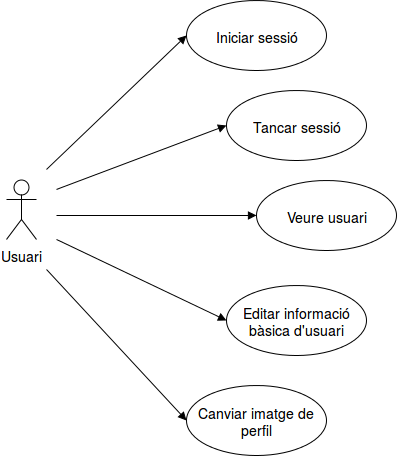
\includegraphics[scale=0.6]{Figures/casosUs_gestioUsuaris.png}
\caption{Diagrama de casos d'ús referent a la gestió d'usuaris}
\end{figure}

\begin{table}[!h]
\centering
\begin{tabular}{|l|L|l|}
\hline
\textbf{Cas d'ús}& \#1 & Iniciar sessió \\ \hline
\textbf{Actor principal} & \multicolumn{2}{l|}{Usuari} \\ \hline
\textbf{Precondició} & \multicolumn{2}{M|}{L'usuari ha accedit a la primera pantalla de l'aplicació.} \\ \hline
\textbf{Trigger} & \multicolumn{2}{M|}{L'usuari vol iniciar sessió al sistema.} \\ \hline
\multicolumn{3}{|T|}{\textbf{Escenari principal d'èxit}} \\ \hline
\multicolumn{3}{|T|}{1. L'usuari clica al botó d'iniciar sessió.}\\
\multicolumn{3}{|T|}{2. El sistema redirigeix l'usuari al llistat de comptes de Google disponibles al dispositiu.}\\
\multicolumn{3}{|T|}{3. L'usuari selecciona el compte desitjat.}\\
\multicolumn{3}{|T|}{4. El sistema redirigeix a l'usuari a la pantalla principal de l'aplicació, ja amb la sessió iniciada.}\\
\hline
\end{tabular}
\label{}
\caption{Cas d'ús \textit{Iniciar sessió}}
\end{table}

\begin{table}[!h]
\centering
\begin{tabular}{|l|L|l|}
\hline
\textbf{Cas d'ús}& \#2 & Tancar sessió \\ \hline
\textbf{Actor principal} & \multicolumn{2}{l|}{Usuari} \\ \hline
\textbf{Precondició} & \multicolumn{2}{M|}{L'usuari ha accedit a la pantalla principal de l'aplicació.} \\ \hline
\textbf{Trigger} & \multicolumn{2}{M|}{L'usuari vol tancar sessió al sistema.} \\ \hline
\multicolumn{3}{|T|}{\textbf{Escenari principal d'èxit}} \\ \hline
\multicolumn{3}{|T|}{1. L'usuari clica sobre la icona de la cantonada esquerra de la barra superior.}\\
\multicolumn{3}{|T|}{2. El sistema mostra a l'usuari un desplegable amb l'opció de tancar sessió.}\\
\multicolumn{3}{|T|}{3. L'usuari clica sobre l'opció de tancar sessió}\\
\multicolumn{3}{|T|}{4. El sistema redirigeix a l'usuari a la primera pantalla de l'aplicació, ja amb la sessió tancada}\\
\hline
\end{tabular}
\label{}
\caption{Cas d'ús \textit{Tancar sessió}}
\end{table}

\begin{table}[!h]
\centering
\begin{tabular}{|l|L|l|}
\hline
\textbf{Cas d'ús}& \#3 & Veure usuari \\ \hline
\textbf{Actor principal} & \multicolumn{2}{l|}{Usuari} \\ \hline
\textbf{Precondició} & \multicolumn{2}{M|}{L'usuari ha accedit a la pantalla principal de l'aplicació.} \\ \hline
\textbf{Trigger} & \multicolumn{2}{M|}{L'usuari vol accedir a la seva informació.} \\ \hline
\multicolumn{3}{|T|}{\textbf{Escenari principal d'èxit}} \\ \hline
\multicolumn{3}{|T|}{1. L'usuari clica sobre el \textit{Navigational drawer} amb l'objectiu de fer-lo desplegar.}\\
\multicolumn{3}{|T|}{2. El sistema desplega el menú lateral.}\\
\multicolumn{3}{|T|}{3. L'usuari clica sobre la seva imatge situada a la part superior del menú lateral.}\\
\multicolumn{3}{|T|}{4. El sistema redirigeix a l'usuari a la pantalla de detall d'usuari.}\\
\hline
\end{tabular}
\label{}
\caption{Cas d'ús \textit{Veure usuari}}
\end{table}

\begin{table}[!h]
\centering
\begin{tabular}{|l|L|l|}
\hline
\textbf{Cas d'ús}& \#4 & Editar informació bàsica d'usuari \\ \hline
\textbf{Actor principal} & \multicolumn{2}{l|}{Usuari} \\ \hline
\textbf{Precondició} & \multicolumn{2}{M|}{L'usuari ha accedit a la pantalla de detall de l'usuari.} \\ \hline
\textbf{Trigger} & \multicolumn{2}{M|}{L'usuari vol modificar la seva informació bàsica.} \\ \hline
\multicolumn{3}{|T|}{\textbf{Escenari principal d'èxit}} \\ \hline
\multicolumn{3}{|T|}{1. L'usuari clica sobre el botó rodó de la dreta de la part inferior de la pantalla.}\\
\multicolumn{3}{|T|}{2. El sistema redirigeix a l'usuari a la pantalla d'editar usuari.}\\
\multicolumn{3}{|T|}{3. L'usuari modifica algun o alguns dels tres camps que té disponibles: nom, cognom i localització. L'usuari clica sobre el botó superior de la dreta per confirmar els canvis.}\\
\multicolumn{3}{|T|}{4. El sistema emmagatzema els canvis i redirigeix a l'usuari a la pantalla de detall d'usuari.}\\
\hline
\multicolumn{3}{|T|}{\textbf{Extensions}} \\ \hline
\multicolumn{3}{|T|}{2.a L'usuari cancel·la els canvis} \\
\multicolumn{3}{|T|}{\tab2.a.1 L'usuari clica sobre la marxa enrere de la barra superior.} \\
\multicolumn{3}{|T|}{\tab2.a.2 El sistema redirigeix a l'usuari a la pantalla de detall de l'usuari sense cap canvi emmagatzemat.} \\\hline
\end{tabular}
\label{}
\caption{Cas d'ús \textit{Editar informació bàsica d'usuari}}
\end{table}

\begin{table}[!h]
\centering
\begin{tabular}{|l|L|l|}
\hline
\textbf{Cas d'ús}& \#5 & Canviar imatge de perfil \\ \hline
\textbf{Actor principal} & \multicolumn{2}{l|}{Usuari} \\ \hline
\textbf{Precondició} & \multicolumn{2}{M|}{L'usuari ha accedit a la pantalla de detall de l'usuari.} \\ \hline
\textbf{Trigger} & \multicolumn{2}{M|}{L'usuari vol modificar la seva imatge de perfil.} \\ \hline
\multicolumn{3}{|T|}{\textbf{Escenari principal d'èxit}} \\ \hline
\multicolumn{3}{|T|}{1. L'usuari clica sobre el botó rodó de la dreta de la part inferior de la pantalla.}\\
\multicolumn{3}{|T|}{2. El sistema redirigeix a l'usuari a la pantalla d'editar usuari.}\\
\multicolumn{3}{|T|}{3. L'usuari clica sobre la imatge d'usuari.}\\
\multicolumn{3}{|T|}{4. El sistema mostra la galeria amb les imatges disponibles dins del dispositiu.}\\
\multicolumn{3}{|T|}{5. L'usuari selecciona la imatge desitjada.}\\
\multicolumn{3}{|T|}{6. El sistema redirigeix a la pantalla d'editar usuari amb la imatge modificada per la seleccionada.}\\
\multicolumn{3}{|T|}{7. L'usuari clica sobre el botó superior de la dreta per confirmar els canvis.}\\
\multicolumn{3}{|T|}{8. El sistema emmagatzema els canvis i redirigeix a l'usuari a la pantalla de detall d'usuari.}\\
\hline
\multicolumn{3}{|T|}{\textbf{Extensions}} \\ \hline
\multicolumn{3}{|T|}{2.a L'usuari cancel·la els canvis} \\
\multicolumn{3}{|T|}{\tab2.a.1 L'usuari clica sobre la marxa enrere de la barra superior.} \\
\multicolumn{3}{|T|}{\tab2.a.2 El sistema redirigeix a l'usuari a la pantalla de detall de l'usuari sense cap canvi emmagatzemat.} \\
\multicolumn{3}{|T|}{6.a L'usuari cancel·la els canvis} \\
\multicolumn{3}{|T|}{\tab6.a.1 L'usuari clica sobre la marxa enrere de la barra superior.} \\
\multicolumn{3}{|T|}{\tab6.a.2 El sistema redirigeix a l'usuari a la pantalla de detall de l'usuari sense cap canvi emmagatzemat.} \\\hline
\end{tabular}
\label{}
\caption{Cas d'ús \textit{Canviar imatge de perfil}}
\end{table}

\clearpage
\subsection{Gestió de l'establiment}
\begin{figure}[H]
\centering
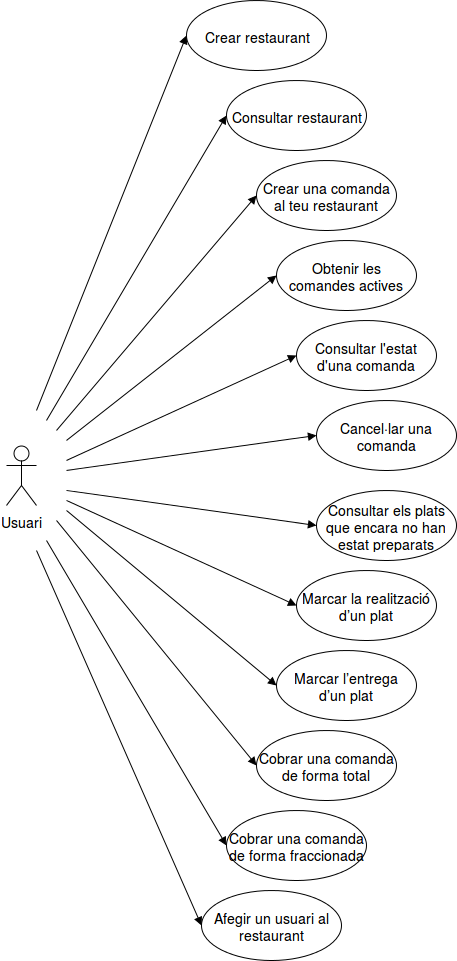
\includegraphics[scale=0.6]{Figures/casosUs_gestioEstabliment.png}
\caption{Diagrama de casos d'ús referent a la gestió de l'establiment}
\end{figure}

\begin{table}[!h]
\centering
\begin{tabular}{|l|L|l|}
\hline
\textbf{Cas d'ús}& \#6 & Crear restaurant \\ \hline
\textbf{Actor principal} & \multicolumn{2}{l|}{Usuari} \\ \hline
\textbf{Precondició} & \multicolumn{2}{M|}{L'usuari ha accedit a la pantalla principal de l'aplicació.} \\ \hline
\textbf{Trigger} & \multicolumn{2}{M|}{L'usuari vol crear un restaurant amb tots els seus detalls i informació.} \\ \hline
\multicolumn{3}{|T|}{\textbf{Escenari principal d'èxit}} \\ \hline
\multicolumn{3}{|T|}{1. L'usuari clica sobre el \textit{Navigational drawer} amb l'objectiu de fer-lo desplegar.}\\
\multicolumn{3}{|T|}{2. El sistema desplega el menú lateral.}\\
\multicolumn{3}{|T|}{3. L'usuari clica sobre la pestanya anomenada \textit{Create restaurant} situada a la part superior del menú lateral.}\\
\multicolumn{3}{|T|}{4. El sistema redirigeix a l'usuari a la pantalla de creació del restaurant.}\\
\multicolumn{3}{|T|}{5. L'usuari completa tots els camps disponibles (nom, descripció, localització, telèfon de contacte, pàgina web i nombre de taules) i després acciona el botó de següent situat a la part inferior-dreta.}\\
\multicolumn{3}{|T|}{6. El sistema redirigeix a l'usuari a la pantalla de creació d'horaris d'apertura.}\\
\multicolumn{3}{|T|}{7. L'usuari completa l'horari d'apertura i de clausura dels set dies de la setmana, i acciona el botó de següent situat a la part inferior-dreta.}\\
\multicolumn{3}{|T|}{8. El sistema redirigeix a l'usuari a la pantalla de creació de plats i menús.}\\
\multicolumn{3}{|T|}{9. L'usuari crea plats i menús accionant sobre l'opció especifica del menú desplegable de la part inferior-dreta especificant el nom, la descripció i el preu, i el conjunt de plats en cas del menú. Un cop finalitzat, l'usuari acciona el botó de la part superior-dreta per finalitzar la creació del restaurant. }\\
\multicolumn{3}{|T|}{10. El sistema redirigeix a l'usuari a la pantalla principal de l'aplicació, ja amb el restaurant creat i vinculat amb l'usuari actual.}\\
\hline
\multicolumn{3}{|T|}{\textbf{Extensions}} \\ \hline
\multicolumn{3}{|T|}{5.a L'usuari cancel·la els canvis en la informació bàsica} \\
\multicolumn{3}{|T|}{\tab5.a.1 L'usuari clica sobre la marxa enrere de la barra superior.} \\
\multicolumn{3}{|T|}{\tab5.a.2 El sistema redirigeix a l'usuari a la pantalla principal de l'aplicació sense cap canvi emmagatzemat.} \\
\multicolumn{3}{|T|}{7.a L'usuari cancel·la els canvis en l'apertura del restaurant} \\
\multicolumn{3}{|T|}{\tab7.a.1 L'usuari clica sobre la marxa enrere de la barra superior.} \\
\multicolumn{3}{|T|}{\tab7.a.2 El sistema redirigeix a l'usuari a la pantalla d'informació bàsica del restaurant sense cap canvi emmagatzemat.} \\
\multicolumn{3}{|T|}{9.a L'usuari cancel·la els canvis en la creació dels plats i menús} \\
\multicolumn{3}{|T|}{\tab9.a.1 L'usuari clica sobre la marxa enrere de la barra superior.} \\
\multicolumn{3}{|T|}{\tab9.a.2 El sistema redirigeix a l'usuari a la pantalla d'horaris d'apertura del restaurant sense cap canvi emmagatzemat.} \\
\hline
\end{tabular}
\label{}
\caption{Cas d'ús \textit{Crear restaurant}}
\end{table}

\begin{table}[!h]
\centering
\begin{tabular}{|l|L|l|}
\hline
\textbf{Cas d'ús}& \#7 & Consultar restaurant \\ \hline
\textbf{Actor principal} & \multicolumn{2}{l|}{Usuari} \\ \hline
\textbf{Precondició} & \multicolumn{2}{M|}{L'usuari ha accedit a la pantalla principal de l'aplicació.} \\ \hline
\textbf{Trigger} & \multicolumn{2}{M|}{L'usuari vol consultar el seu restaurant.} \\ \hline
\multicolumn{3}{|T|}{\textbf{Escenari principal d'èxit}} \\ \hline
\multicolumn{3}{|T|}{1. L'usuari clica sobre el \textit{Navigational drawer} amb l'objectiu de fer-lo desplegar.}\\
\multicolumn{3}{|T|}{2. El sistema desplega el menú lateral.}\\
\multicolumn{3}{|T|}{3. L'usuari clica sobre la pestanya anomenada \textit{See restaurant} del menú lateral.}\\
\multicolumn{3}{|T|}{4. El sistema redirigeix a l'usuari a la pantalla de vista del restaurant.}\\
\hline
\end{tabular}
\label{}
\caption{Cas d'ús \textit{Consultar restaurant}}
\end{table}

\begin{table}[!h]
\centering
\begin{tabular}{|l|L|l|}
\hline
\textbf{Cas d'ús}& \#8 & Crear una comanda al teu restaurant \\ \hline
\textbf{Actor principal} & \multicolumn{2}{l|}{Usuari} \\ \hline
\textbf{Precondició} & \multicolumn{2}{M|}{L'usuari ha accedit a la pantalla de comandes actives.} \\ \hline
\textbf{Trigger} & \multicolumn{2}{M|}{L'usuari vol crear una comanda al seu restaurant amb tots els detalls que la caracteritzen.} \\ \hline
\multicolumn{3}{|T|}{\textbf{Escenari principal d'èxit}} \\ \hline
\multicolumn{3}{|T|}{1. L'usuari clica sobre el botó rodó de la part de la part inferior de la pantalla.}\\
\multicolumn{3}{|T|}{2. El sistema mostra un desplegable amb un petit formulari per introduir la taula a on es realitza la comanda.}\\
\multicolumn{3}{|T|}{3. L'usuari escriu el número de taula a on es realitza la comanda i prem \textit{Acceptar}.}\\
\multicolumn{3}{|T|}{4. El sistema redirigeix a l'usuari a la pantalla de creació de comanda.}\\
\multicolumn{3}{|T|}{5. L'usuari selecciona els plats i menús que desitja el client prement el botó de \textit{+} de cada un dels ítems de la carta. En cas que estiguem parlant d'un menú, s'haurà de seleccionar quins plats es vol del menú determinat. Un cop tot completat, l'usuari clica sobre el botó de la part superior-dreta per finalitzar la creació de la comanda.}\\
\multicolumn{3}{|T|}{6. El sistema redirigeix a l'usuari a la pantalla de comandes actives amb la nova comanda emmagatzemada.}\\
\hline
\multicolumn{3}{|T|}{\textbf{Extensions}} \\ \hline
\multicolumn{3}{|T|}{5.a L'usuari cancel·la els canvis} \\
\multicolumn{3}{|T|}{\tab5.a.1 L'usuari clica sobre la marxa enrere de la barra superior.} \\
\multicolumn{3}{|T|}{\tab5.a.2 El sistema redirigeix a l'usuari a la pantalla de comandes actives sense cap canvi emmagatzemat.} \\\hline
\end{tabular}
\label{}
\caption{Cas d'ús \textit{Crear una comanda al teu restaurant}}
\end{table}

\begin{table}[!h]
\centering
\begin{tabular}{|l|L|l|}
\hline
\textbf{Cas d'ús}& \#9 & Obtenir les comandes actives \\ \hline
\textbf{Actor principal} & \multicolumn{2}{l|}{Usuari} \\ \hline
\textbf{Precondició} & \multicolumn{2}{M|}{L'usuari ha accedit a la pantalla principal de l'aplicació.} \\ \hline
\textbf{Trigger} & \multicolumn{2}{M|}{L'usuari vol consultar les comandes actives.} \\ \hline
\multicolumn{3}{|T|}{\textbf{Escenari principal d'èxit}} \\ \hline
\multicolumn{3}{|T|}{1. L'usuari clica sobre el \textit{Navigational drawer} amb l'objectiu de fer-lo desplegar.}\\
\multicolumn{3}{|T|}{2. El sistema desplega el menú lateral.}\\
\multicolumn{3}{|T|}{3. L'usuari clica sobre la pestanya anomenada \textit{Active orders} del menú lateral.}\\
\multicolumn{3}{|T|}{4. El sistema redirigeix a l'usuari a la pantalla de comandes actives del restaurant.}\\
\hline
\end{tabular}
\label{}
\caption{Cas d'ús \textit{Obtenir les comandes actives}}
\end{table}

\begin{table}[!h]
\centering
\begin{tabular}{|l|L|l|}
\hline
\textbf{Cas d'ús}& \#10 & Consultar l'estat d'una comanda \\ \hline
\textbf{Actor principal} & \multicolumn{2}{l|}{Usuari} \\ \hline
\textbf{Precondició} & \multicolumn{2}{M|}{L'usuari ha accedit a la pantalla de comandes actives.} \\ \hline
\textbf{Trigger} & \multicolumn{2}{M|}{L'usuari vol consultar l'estat d'una comanda.} \\ \hline
\multicolumn{3}{|T|}{\textbf{Escenari principal d'èxit}} \\ \hline
\multicolumn{3}{|T|}{1. L'usuari clica sobre alguna de les comandes que disposa en el llistat.}\\
\multicolumn{3}{|T|}{2. El sistema redirigeix a l'usuari a la vista de detall de la comanda.}\\
\hline
\end{tabular}
\label{}
\caption{Cas d'ús \textit{Consultar l'estat d'una comanda}}
\end{table}

\begin{table}[!h]
\centering
\begin{tabular}{|l|L|l|}
\hline
\textbf{Cas d'ús}& \#11 & Cancel·lar una comanda \\ \hline
\textbf{Actor principal} & \multicolumn{2}{l|}{L'usuari ha accedit a la pantalla de detall de la comanda.} \\ \hline
\textbf{Trigger} & \multicolumn{2}{M|}{L'usuari vol cancel·lar una comanda.} \\ \hline
\multicolumn{3}{|T|}{\textbf{Escenari principal d'èxit}} \\ \hline
\multicolumn{3}{|T|}{1. L'usuari clica sobre la icona de la cantonada esquerra de la barra superior.}\\
\multicolumn{3}{|T|}{2. El sistema mostra a l'usuari un desplegable amb l'opció de cancel·lar la comanda.}\\
\multicolumn{3}{|T|}{3. L'usuari clica sobre l'opció de cancel·lar comanda}\\
\multicolumn{3}{|T|}{4. El sistema redirigeix a l'usuari a la pantalla principal de l'aplicació, ja amb la comanda cancel·lada}\\
\hline
\end{tabular}
\label{}
\caption{Cas d'ús \textit{Cancel·lar una comanda}}
\end{table}

\begin{table}[!h]
\centering
\begin{tabular}{|l|L|l|}
\hline
\textbf{Cas d'ús}& \#12 & Consultar els plats que encara no han estat preparats \\ \hline
\textbf{Actor principal} & \multicolumn{2}{l|}{Usuari} \\ \hline
\textbf{Precondició} & \multicolumn{2}{M|}{L'usuari ha accedit a la pantalla principal de l'aplicació.} \\ \hline
\textbf{Trigger} & \multicolumn{2}{M|}{L'usuari vol consultar els plats que encara no han estat preparats.} \\ \hline
\multicolumn{3}{|T|}{\textbf{Escenari principal d'èxit}} \\ \hline
\multicolumn{3}{|T|}{1. L'usuari clica sobre el \textit{Navigational drawer} amb l'objectiu de fer-lo desplegar.}\\
\multicolumn{3}{|T|}{2. El sistema desplega el menú lateral.}\\
\multicolumn{3}{|T|}{3. L'usuari clica sobre la pestanya anomenada \textit{Kitchen} del menú lateral.}\\
\multicolumn{3}{|T|}{4. El sistema redirigeix a l'usuari a la pantalla de cuina.}\\
\hline
\end{tabular}
\label{}
\caption{Cas d'ús \textit{Consultar els plats que encara no han estat preparats}}
\end{table}

\begin{table}[!h]
\centering
\begin{tabular}{|l|L|l|}
\hline
\textbf{Cas d'ús}& \#13 & Marcar la realització d'un plat \\ \hline
\textbf{Actor principal} & \multicolumn{2}{l|}{Usuari} \\ \hline
\textbf{Precondició} & \multicolumn{2}{M|}{L'usuari ha accedit a la pantalla de cuina.} \\ \hline
\textbf{Trigger} & \multicolumn{2}{M|}{L'usuari vol marcar la realització d'un plat no preparat.} \\ \hline
\multicolumn{3}{|T|}{\textbf{Escenari principal d'èxit}} \\ \hline
\multicolumn{3}{|T|}{1. L'usuari selecciona l'ítem que ja ha preparat i confirma la seva elecció prement \textit{Acceptar}.}\\
\multicolumn{3}{|T|}{2. El sistema emmagatzema el canvi i elimina l'ítem del llistat.}\\
\hline
\end{tabular}
\label{}
\caption{Cas d'ús \textit{Marcar la realització d'un plat}}
\end{table}

\begin{table}[!h]
\centering
\begin{tabular}{|l|L|l|}
\hline
\textbf{Cas d'ús}& \#14 & Marcar l'entrega d'un plat \\ \hline
\textbf{Actor principal} & \multicolumn{2}{l|}{Usuari} \\ \hline
\textbf{Precondició} & \multicolumn{2}{M|}{L'usuari ha accedit a la pantalla de detall de la comanda.} \\ \hline
\textbf{Trigger} & \multicolumn{2}{M|}{L'usuari vol marcar l'entrega d'un plat.} \\ \hline
\multicolumn{3}{|T|}{\textbf{Escenari principal d'èxit}} \\ \hline
\multicolumn{3}{|T|}{1. L'usuari selecciona el botó rodó vinculat amb l'ítem desitjat i que vol marcar com a entregat.}\\
\multicolumn{3}{|T|}{2. El sistema emmagatzema el canvi.}\\
\hline
\end{tabular}
\label{}
\caption{Cas d'ús \textit{Marcar l'entrega d'un plat}}
\end{table}

\begin{table}[!h]
\centering
\begin{tabular}{|l|L|l|}
\hline
\textbf{Cas d'ús}& \#15 & Cobrar una comanda de forma total \\ \hline
\textbf{Actor principal} & \multicolumn{2}{l|}{Usuari} \\ \hline
\textbf{Precondició} & \multicolumn{2}{M|}{L'usuari ha accedit a la pantalla de detall de la comanda.} \\ \hline
\textbf{Trigger} & \multicolumn{2}{M|}{L'usuari vol cobrar una comanda de forma total.} \\ \hline
\multicolumn{3}{|T|}{\textbf{Escenari principal d'èxit}} \\ \hline
\multicolumn{3}{|T|}{1. L'usuari clica al botó rodó de la part inferior-dreta de la pantalla.}\\
\multicolumn{3}{|T|}{2. El sistema mostra un diàleg en el qual et permet elegir fer el cobrament parcialment o no.}\\
\multicolumn{3}{|T|}{3. L'usuari clica sobre \textit{All}.}\\
\multicolumn{3}{|T|}{4. El sistema tanca el diàleg i en mostra un altre confirmant la recol·lecta del total de la comanda.}\\
\multicolumn{3}{|T|}{5. L'usuari clica sobre \textit{Yes}.}\\
\multicolumn{3}{|T|}{6. El sistema tanca el diàleg i emmagatzema les dades marcant com a cobrada la comanda corresponent.}\\
\hline
\end{tabular}
\label{}
\caption{Cas d'ús \textit{Cobrar una comanda de forma total}}
\end{table}

\begin{table}[!h]
\centering
\begin{tabular}{|l|L|l|}
\hline
\textbf{Cas d'ús}& \#16 & Cobrar una comanda de forma fraccionada \\ \hline
\textbf{Actor principal} & \multicolumn{2}{l|}{Usuari} \\ \hline
\textbf{Precondició} & \multicolumn{2}{M|}{L'usuari ha accedit a la pantalla de detall de la comanda.} \\ \hline
\textbf{Trigger} & \multicolumn{2}{M|}{L'usuari vol cobrar una comanda de forma fraccionada.} \\ \hline
\multicolumn{3}{|T|}{\textbf{Escenari principal d'èxit}} \\ \hline
\multicolumn{3}{|T|}{1. L'usuari clica al botó rodó de la part inferior-dreta de la pantalla.}\\
\multicolumn{3}{|T|}{2. El sistema mostra un diàleg en el qual et permet elegir fer el cobrament parcialment o no.}\\
\multicolumn{3}{|T|}{3. L'usuari clica sobre \textit{In groups}.}\\
\multicolumn{3}{|T|}{4. El sistema tanca el diàleg i mostra tots els ítems que encara no han estat cobrats de la comanda.}\\
\multicolumn{3}{|T|}{5. L'usuari selecciona els ítems que vol cobrar i clica sobre el botó rodó de la part inferior de la pantalla.}\\
\multicolumn{3}{|T|}{6. El sistema mostra un diàleg confirmant la recol·lecta dels elements seleccionats dins la comanda.}\\
\multicolumn{3}{|T|}{7. L'usuari clica sobre \textit{Yes}.}\\
\multicolumn{3}{|T|}{8. El sistema tanca el diàleg i emmagatzema les dades marcant com a cobrats els plats corresponents.}\\
\hline
\end{tabular}
\label{}
\caption{Cas d'ús \textit{Cobrar una comanda de forma fraccionada}}
\end{table}

\begin{table}[!h]
\centering
\begin{tabular}{|l|L|l|}
\hline
\textbf{Cas d'ús}& \#17 & Afegir un usuari al restaurant \\ \hline
\textbf{Actor principal} & \multicolumn{2}{l|}{Usuari} \\ \hline
\textbf{Precondició} & \multicolumn{2}{M|}{L'usuari ha accedit a la pantalla de detall del restaurant.} \\ \hline
\textbf{Trigger} & \multicolumn{2}{M|}{L'usuari vol afegir un usuari dins de l'equip del restaurant.} \\ \hline
\multicolumn{3}{|T|}{\textbf{Escenari principal d'èxit}} \\ \hline
\multicolumn{3}{|T|}{1. L'usuari clica sobre el botó rodó de la barra superior.}\\
\multicolumn{3}{|T|}{2. El sistema mostra un diàleg amb un petit formulari per introduir l'adreça de correu electrònic de l'usuari a afegir.}\\
\multicolumn{3}{|T|}{3. L'usuari escriu l'adreça de correu electrònic de l'usuari a afegir.}\\
\multicolumn{3}{|T|}{4. El sistema emmagatzema la informació i tanca el diàleg.}\\
\hline
\multicolumn{3}{|T|}{\textbf{Extensions}} \\ \hline
\multicolumn{3}{|T|}{3.a L'usuari no existeix} \\
\multicolumn{3}{|T|}{\tab3.a.1 L'usuari introdueix una adreça electrònica no registrada a la base de dades de la plataforma.} \\
\multicolumn{3}{|T|}{\tab3.a.2 El sistema reporta la incidència a l'usuari i tanca el diàleg sense cap canvi en la persistència de la plataforma.} \\
\multicolumn{3}{|T|}{3.b L'usuari ja pertany a un restaurant} \\
\multicolumn{3}{|T|}{\tab3.b.1 L'usuari introdueix una adreça electrònica pertanyent a un usuari que ja està vinculat a un restaurant.} \\
\multicolumn{3}{|T|}{\tab3.b.2 El sistema reporta la incidència a l'usuari i tanca el diàleg sense cap canvi en la persistència de la plataforma.} \\
\hline
\end{tabular}
\label{}
\caption{Cas d'ús \textit{Afegir un usuari al restaurant}}
\end{table}

\clearpage
\subsection{Anàlisi de l'establiment}
\begin{figure}[H]
\centering
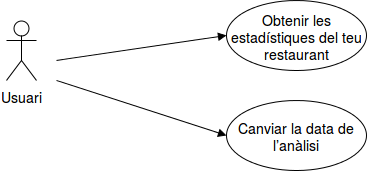
\includegraphics[scale=0.6]{Figures/casosUs_analisiEstabliment.png}
\caption{Diagrama de casos d'ús referent a l'anàlisi de l'establiment}
\end{figure}

\begin{table}[!h]
\centering
\begin{tabular}{|l|L|l|}
\hline
\textbf{Cas d'ús}& \#18 & Obtenir les estadístiques del teu restaurant  \\ \hline
\textbf{Actor principal} & \multicolumn{2}{l|}{Usuari} \\ \hline
\textbf{Precondició} & \multicolumn{2}{M|}{L'usuari ha accedit a la pantalla principal de l'aplicació.} \\ \hline
\textbf{Trigger} & \multicolumn{2}{M|}{L'usuari vol consultar les estadístiques del seu restaurant.} \\ \hline
\multicolumn{3}{|T|}{\textbf{Escenari principal d'èxit}} \\ \hline
\multicolumn{3}{|T|}{1. L'usuari clica sobre el \textit{Navigational drawer} amb l'objectiu de fer-lo desplegar.}\\
\multicolumn{3}{|T|}{2. El sistema desplega el menú lateral.}\\
\multicolumn{3}{|T|}{3. L'usuari clica sobre la pestanya anomenada \textit{Analytics} del menú lateral.}\\
\multicolumn{3}{|T|}{4. El sistema redirigeix a l'usuari a la pantalla d'estadístiques.}\\
\hline
\end{tabular}
\label{}
\caption{Cas d'ús \textit{Obtenir les estadístiques del teu restaurant}}
\end{table}

\begin{table}[!h]
\centering
\begin{tabular}{|l|L|l|}
\hline
\textbf{Cas d'ús}& \#19 & Canviar la data de l'anàlisi  \\ \hline
\textbf{Actor principal} & \multicolumn{2}{l|}{Usuari} \\ \hline
\textbf{Precondició} & \multicolumn{2}{M|}{L'usuari ha accedit a la pantalla d'estadístiques.} \\ \hline
\textbf{Trigger} & \multicolumn{2}{M|}{L'usuari vol canviar la data de visualització per analitzar les estadístiques d'un altre període.} \\ \hline
\multicolumn{3}{|T|}{\textbf{Escenari principal d'èxit}} \\ \hline
\multicolumn{3}{|T|}{1. L'usuari clica sobre el botó amb icona de calendari situat a la barra superior.}\\
\multicolumn{3}{|T|}{2. El sistema mostra un diàleg amb un calendari per seleccionar una data.}\\ 
\multicolumn{3}{|T|}{3. L'usuari selecciona un dia del calendari i prem \textit{Acceptar}.}\\ 
\multicolumn{3}{|T|}{4. El sistema refresca la vista amb la nova data seleccionada i tanca el diàleg.}\\ 
\hline
\end{tabular}
\label{}
\caption{Cas d'ús \textit{Canviar la data de l'anàlisi}}
\end{table}

\clearpage
\subsection{Interacció del client}
\begin{figure}[H]
\centering
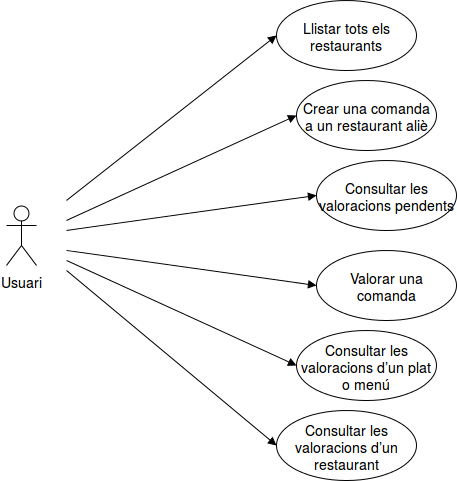
\includegraphics[scale=0.6]{Figures/casosUs_interaccioClient.png}
\caption{Diagrama de casos d'ús referent a la interacció del client}
\end{figure}

\begin{table}[!h]
\centering
\begin{tabular}{|l|L|l|}
\hline
\textbf{Cas d'ús}& \#20 & Llistar tots els restaurants  \\ \hline
\textbf{Actor principal} & \multicolumn{2}{l|}{Usuari} \\ \hline
\textbf{Precondició} & \multicolumn{2}{M|}{TEST} \\ \hline
\textbf{Trigger} & \multicolumn{2}{M|}{TEST} \\ \hline
\multicolumn{3}{|T|}{\textbf{Escenari principal d'èxit}} \\ \hline
\multicolumn{3}{|T|}{1. TEST}\\
\multicolumn{3}{|T|}{2. TEST}\\ 
\multicolumn{3}{|T|}{3. TEST}\\ 
\multicolumn{3}{|T|}{4. TEST}\\ 
\hline
\multicolumn{3}{|T|}{\textbf{Extensions}} \\ \hline
\multicolumn{3}{|T|}{3.a TEST} \\ 
\multicolumn{3}{|T|}{\tab3.a.1  TEST} \\
\multicolumn{3}{|T|}{\tab3.a.2  TEST} \\
\multicolumn{3}{|T|}{4.a TEST} \\
\multicolumn{3}{|T|}{\tab4.a.1 TEST} \\ 
\multicolumn{3}{|T|}{\tab4.a.2 TEST} \\\hline
\end{tabular}
\label{}
\caption{Cas d'ús \textit{TEST}}
\end{table}

\begin{table}[!h]
\centering
\begin{tabular}{|l|L|l|}
\hline
\textbf{Cas d'ús}& \#21 & Crear una comanda a un restaurant aliè  \\ \hline
\textbf{Actor principal} & \multicolumn{2}{l|}{Usuari} \\ \hline
\textbf{Precondició} & \multicolumn{2}{M|}{TEST} \\ \hline
\textbf{Trigger} & \multicolumn{2}{M|}{TEST} \\ \hline
\multicolumn{3}{|T|}{\textbf{Escenari principal d'èxit}} \\ \hline
\multicolumn{3}{|T|}{1. TEST}\\
\multicolumn{3}{|T|}{2. TEST}\\ 
\multicolumn{3}{|T|}{3. TEST}\\ 
\multicolumn{3}{|T|}{4. TEST}\\ 
\hline
\multicolumn{3}{|T|}{\textbf{Extensions}} \\ \hline
\multicolumn{3}{|T|}{3.a TEST} \\ 
\multicolumn{3}{|T|}{\tab3.a.1  TEST} \\
\multicolumn{3}{|T|}{\tab3.a.2  TEST} \\
\multicolumn{3}{|T|}{4.a TEST} \\
\multicolumn{3}{|T|}{\tab4.a.1 TEST} \\ 
\multicolumn{3}{|T|}{\tab4.a.2 TEST} \\\hline
\end{tabular}
\label{}
\caption{Cas d'ús \textit{TEST}}
\end{table}

\begin{table}[!h]
\centering
\begin{tabular}{|l|L|l|}
\hline
\textbf{Cas d'ús}& \#22 & Consultar les valoracions pendents  \\ \hline
\textbf{Actor principal} & \multicolumn{2}{l|}{Usuari} \\ \hline
\textbf{Precondició} & \multicolumn{2}{M|}{TEST} \\ \hline
\textbf{Trigger} & \multicolumn{2}{M|}{TEST} \\ \hline
\multicolumn{3}{|T|}{\textbf{Escenari principal d'èxit}} \\ \hline
\multicolumn{3}{|T|}{1. TEST}\\
\multicolumn{3}{|T|}{2. TEST}\\ 
\multicolumn{3}{|T|}{3. TEST}\\ 
\multicolumn{3}{|T|}{4. TEST}\\ 
\hline
\multicolumn{3}{|T|}{\textbf{Extensions}} \\ \hline
\multicolumn{3}{|T|}{3.a TEST} \\ 
\multicolumn{3}{|T|}{\tab3.a.1  TEST} \\
\multicolumn{3}{|T|}{\tab3.a.2  TEST} \\
\multicolumn{3}{|T|}{4.a TEST} \\
\multicolumn{3}{|T|}{\tab4.a.1 TEST} \\ 
\multicolumn{3}{|T|}{\tab4.a.2 TEST} \\\hline
\end{tabular}
\label{}
\caption{Cas d'ús \textit{TEST}}
\end{table}

\begin{table}[!h]
\centering
\begin{tabular}{|l|L|l|}
\hline
\textbf{Cas d'ús}& \#23 & Valorar una comanda  \\ \hline
\textbf{Actor principal} & \multicolumn{2}{l|}{Usuari} \\ \hline
\textbf{Precondició} & \multicolumn{2}{M|}{TEST} \\ \hline
\textbf{Trigger} & \multicolumn{2}{M|}{TEST} \\ \hline
\multicolumn{3}{|T|}{\textbf{Escenari principal d'èxit}} \\ \hline
\multicolumn{3}{|T|}{1. TEST}\\
\multicolumn{3}{|T|}{2. TEST}\\ 
\multicolumn{3}{|T|}{3. TEST}\\ 
\multicolumn{3}{|T|}{4. TEST}\\ 
\hline
\multicolumn{3}{|T|}{\textbf{Extensions}} \\ \hline
\multicolumn{3}{|T|}{3.a TEST} \\ 
\multicolumn{3}{|T|}{\tab3.a.1  TEST} \\
\multicolumn{3}{|T|}{\tab3.a.2  TEST} \\
\multicolumn{3}{|T|}{4.a TEST} \\
\multicolumn{3}{|T|}{\tab4.a.1 TEST} \\ 
\multicolumn{3}{|T|}{\tab4.a.2 TEST} \\\hline
\end{tabular}
\label{}
\caption{Cas d'ús \textit{TEST}}
\end{table}

\begin{table}[!h]
\centering
\begin{tabular}{|l|L|l|}
\hline
\textbf{Cas d'ús}& \#24 & Consultar les valoracions d'un plat o menú  \\ \hline
\textbf{Actor principal} & \multicolumn{2}{l|}{Usuari} \\ \hline
\textbf{Precondició} & \multicolumn{2}{M|}{TEST} \\ \hline
\textbf{Trigger} & \multicolumn{2}{M|}{TEST} \\ \hline
\multicolumn{3}{|T|}{\textbf{Escenari principal d'èxit}} \\ \hline
\multicolumn{3}{|T|}{1. TEST}\\
\multicolumn{3}{|T|}{2. TEST}\\ 
\multicolumn{3}{|T|}{3. TEST}\\ 
\multicolumn{3}{|T|}{4. TEST}\\ 
\hline
\multicolumn{3}{|T|}{\textbf{Extensions}} \\ \hline
\multicolumn{3}{|T|}{3.a TEST} \\ 
\multicolumn{3}{|T|}{\tab3.a.1  TEST} \\
\multicolumn{3}{|T|}{\tab3.a.2  TEST} \\
\multicolumn{3}{|T|}{4.a TEST} \\
\multicolumn{3}{|T|}{\tab4.a.1 TEST} \\ 
\multicolumn{3}{|T|}{\tab4.a.2 TEST} \\\hline
\end{tabular}
\label{}
\caption{Cas d'ús \textit{TEST}}
\end{table}

\begin{table}[!h]
\centering
\begin{tabular}{|l|L|l|}
\hline
\textbf{Cas d'ús}& \#25 & Consultar les valoracions d’un restaurant  \\ \hline
\textbf{Actor principal} & \multicolumn{2}{l|}{Usuari} \\ \hline
\textbf{Precondició} & \multicolumn{2}{M|}{TEST} \\ \hline
\textbf{Trigger} & \multicolumn{2}{M|}{TEST} \\ \hline
\multicolumn{3}{|T|}{\textbf{Escenari principal d'èxit}} \\ \hline
\multicolumn{3}{|T|}{1. TEST}\\
\multicolumn{3}{|T|}{2. TEST}\\ 
\multicolumn{3}{|T|}{3. TEST}\\ 
\multicolumn{3}{|T|}{4. TEST}\\ 
\hline
\multicolumn{3}{|T|}{\textbf{Extensions}} \\ \hline
\multicolumn{3}{|T|}{3.a TEST} \\ 
\multicolumn{3}{|T|}{\tab3.a.1  TEST} \\
\multicolumn{3}{|T|}{\tab3.a.2  TEST} \\
\multicolumn{3}{|T|}{4.a TEST} \\
\multicolumn{3}{|T|}{\tab4.a.1 TEST} \\ 
\multicolumn{3}{|T|}{\tab4.a.2 TEST} \\\hline
\end{tabular}
\label{}
\caption{Cas d'ús \textit{TEST}}
\end{table}